
The aim of this task is to discretize the system dynamics, compute the gradients of the functions and code them.

\section{State space and control inputs}
The system can be modeled as a simple bicycle model,
as shown in Figure \ref{fig:Bicycle}.

\begin{figure}[htp]
\centering
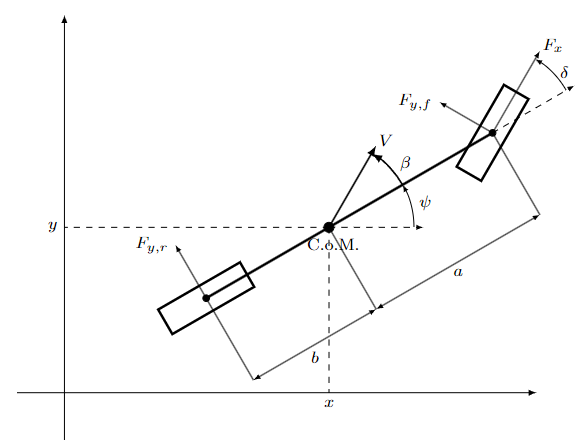
\includegraphics[width=0.5\textwidth]{figs/Bycicle.png}
\caption{Bicycle model}
\label{fig:Bicycle}
\end{figure}

The state space variables are \[ x = [x, y, \psi, V, \beta, \dot{\psi}]^T\] where: $x$ and $y$ represent the position of the center of mass [CoM],
$\psi$ the angle between the horizontal and the chassis, $V$ the velocity of the CoM with respect to the inertial frame, $\beta$ the angle between the chassis and the velocity vector, 
$\dot{\psi}$ the angular rate of changes associated to $\psi$.
The input is \[u = [\delta, F_x]^T\] where $\delta$ is the steering angle and $F_x$ is the force applied by the wheels.

\bigskip
The dynamic model is described by:
\[
\begin{cases}
    \dot{x} &= V\cos\beta\cos\psi - V\sin\beta\sin\psi \\
    \dot{y} &= V\cos\beta\sin\psi + V\sin\beta\cos\psi \\
    m\dot{V} &= F_{y,r} \sin\beta + F_x \cos(\beta - \delta) + F_{y,f}\sin(\beta - \delta) \\
    \dot{\beta} &= \frac{1}{mV}(F_{y,r}\cos\beta + F_{y,f}\cos(\beta - \delta) - F_x\sin(\beta - \delta)) - \dot{\psi} \\
    I_z\ddot{\psi} &= (F_x\sin\delta + F_{y,f}\cos\delta)a - F_{y,r}b\\
\end{cases}
\]

The lateral forces \( F_{y,f} \) and \( F_{y,r} \) can be found as:

\[
\begin{aligned}
    F_{y,f} &= \mu F_{z,f} \beta_f \\
    F_{y,r} &= \mu F_{z,r} \beta_r
\end{aligned}
\]

where \( \beta_f \) and \( \beta_r \) are the front and rear sideslip angles:

\[
\begin{aligned}
    \beta_f = \delta - \frac{V\sin\beta + a\dot{\psi}}{V\cos\beta} \\
    \beta_r = -\frac{V\sin\beta - b\dot{\psi}}{V\cos\beta}
\end{aligned}
\]

The vertical forces on the front and rear wheel can be found as:

\[
\begin{aligned}
    F_{z,f} &= \frac{mgb}{a + b} \\
    F_{z,r} &= \frac{mga}{a + b}
\end{aligned}
\]

The mechanical parameters of the car are: 

\begin{center}
\begin{tabular}{ |c|c|c| } 
 \hline
 m: mass of the car & 1480 & [Kg] \\ 
 $I_z$: inertia of the car & 1950 & $[kg m^2]$ \\ 
 a: distance between rear wheel and CoM & 1.421 & [m]\\ 
 b: distance between front wheel and CoM & 1.029 & [m]\\ 
 $\mu$: friction coefficient & 1 & [nodim]\\ 
 g: acceleration due to gravity & 9.81 & $[m/s^2]$\\ 
 \hline
\end{tabular}
\end{center}


\section{Forward Euler discretization}
In order to write the discrete-time state-space equations, we consider the discrete time version of the bicycle model dynamics, discretized via forward Euler: 
\[
x_{t+1}  = x_t + \delta f_{CT} (x_t, u_t, t)\\
\]

where $\delta > 0$ is a sufficiently small discretization step and $f_{CT} (\cdot,\cdot,\cdot)$ is the continuous-time dynamics. In particular, we choose $\delta = 10^{-2}$. 


We obtain the following discrete-time state-space equations: 
\[
\begin{cases}
    x_{t+1} &= x_t + \delta(V\cos\beta\cos\psi - V\sin\beta\sin\psi) \\
    y_{t+1} &= y_t + \delta(V\cos\beta\sin\psi + V\sin\beta\cos\psi) \\
    \psi_{t+1} &= \psi_t + \delta(\dot{\psi}) \\
    V_{t+1} &= v_t + \delta\left(\frac{1}{m}\left(F_{y,r}\sin\beta + F_x\cos(\beta - \delta) + F_{y,f}\sin(\beta - \delta)\right)\right) \\
    \beta_{t+1} &= \beta_t + \delta\left(\frac{1}{mV}\left(F_{y,r}\cos\beta + F_{y,f}\cos(\beta - \delta) - F_x\sin(\beta - \delta)\right) - (\dot{\psi})\right) \\
    \dot{\psi}_{t+1} &= \dot{\psi}_t + \delta\left(\frac{1}{I_z}\left((F_x\sin\delta + F_{y,f}\cos\delta)a - F_{y,r}b\right)\right)
\end{cases} 
\]

Next, since we are dealing with a non-linear system that is time-invariant, it is necessary to linearize the model by taking its gradient with respect to the state, which is defined as the transpose of the Jacobian Matrix:
\[
    \nabla_1 f(x,u) = \left[\nabla_1 f_1(x,u), \nabla_1 f_2(x,u), \nabla_1 f_3(x,u), \nabla_1 f_4(x,u), \nabla_1 f_5(x,u), \nabla_1 f_6(x,u)\right]
\]

After that, we compute the gradient of our dynamics with respect to our input:
\[
    \nabla_2 f(x,u) = [\nabla_2 f_1(x,u), \nabla_2 f_2(x,u), \nabla_2 f_3(x,u), \nabla_2 f_4(x,u), \nabla_2 f_5(x,u), \nabla_2 f_6(x,u)]
\]

In principle, in order to implement a precise Newton's method, we would also need to compute the Hessian of the dynamics. However, since we used the regularized Newton's method, we don't need these computation as only the hessians of the costs will be needed. We will discuss other implications for this choice in the next chapter. 